\documentclass{article}

\usepackage{graphicx}
\usepackage{tikz}
\usepackage{tikzsymbols}
\usetikzlibrary{calc,patterns,shapes.geometric}
\pagestyle{empty}
\usepackage[margin=0pt]{geometry}
\geometry{papersize={14in,12in}}

\def\centerarc[#1](#2)(#3:#4:#5){\draw[#1] ($(#2)+({#5*cos(#3)},{#5*sin(#3)})$) arc (#3:#4:#5);}

\begin{document}
	\begin{figure}
		\centering
		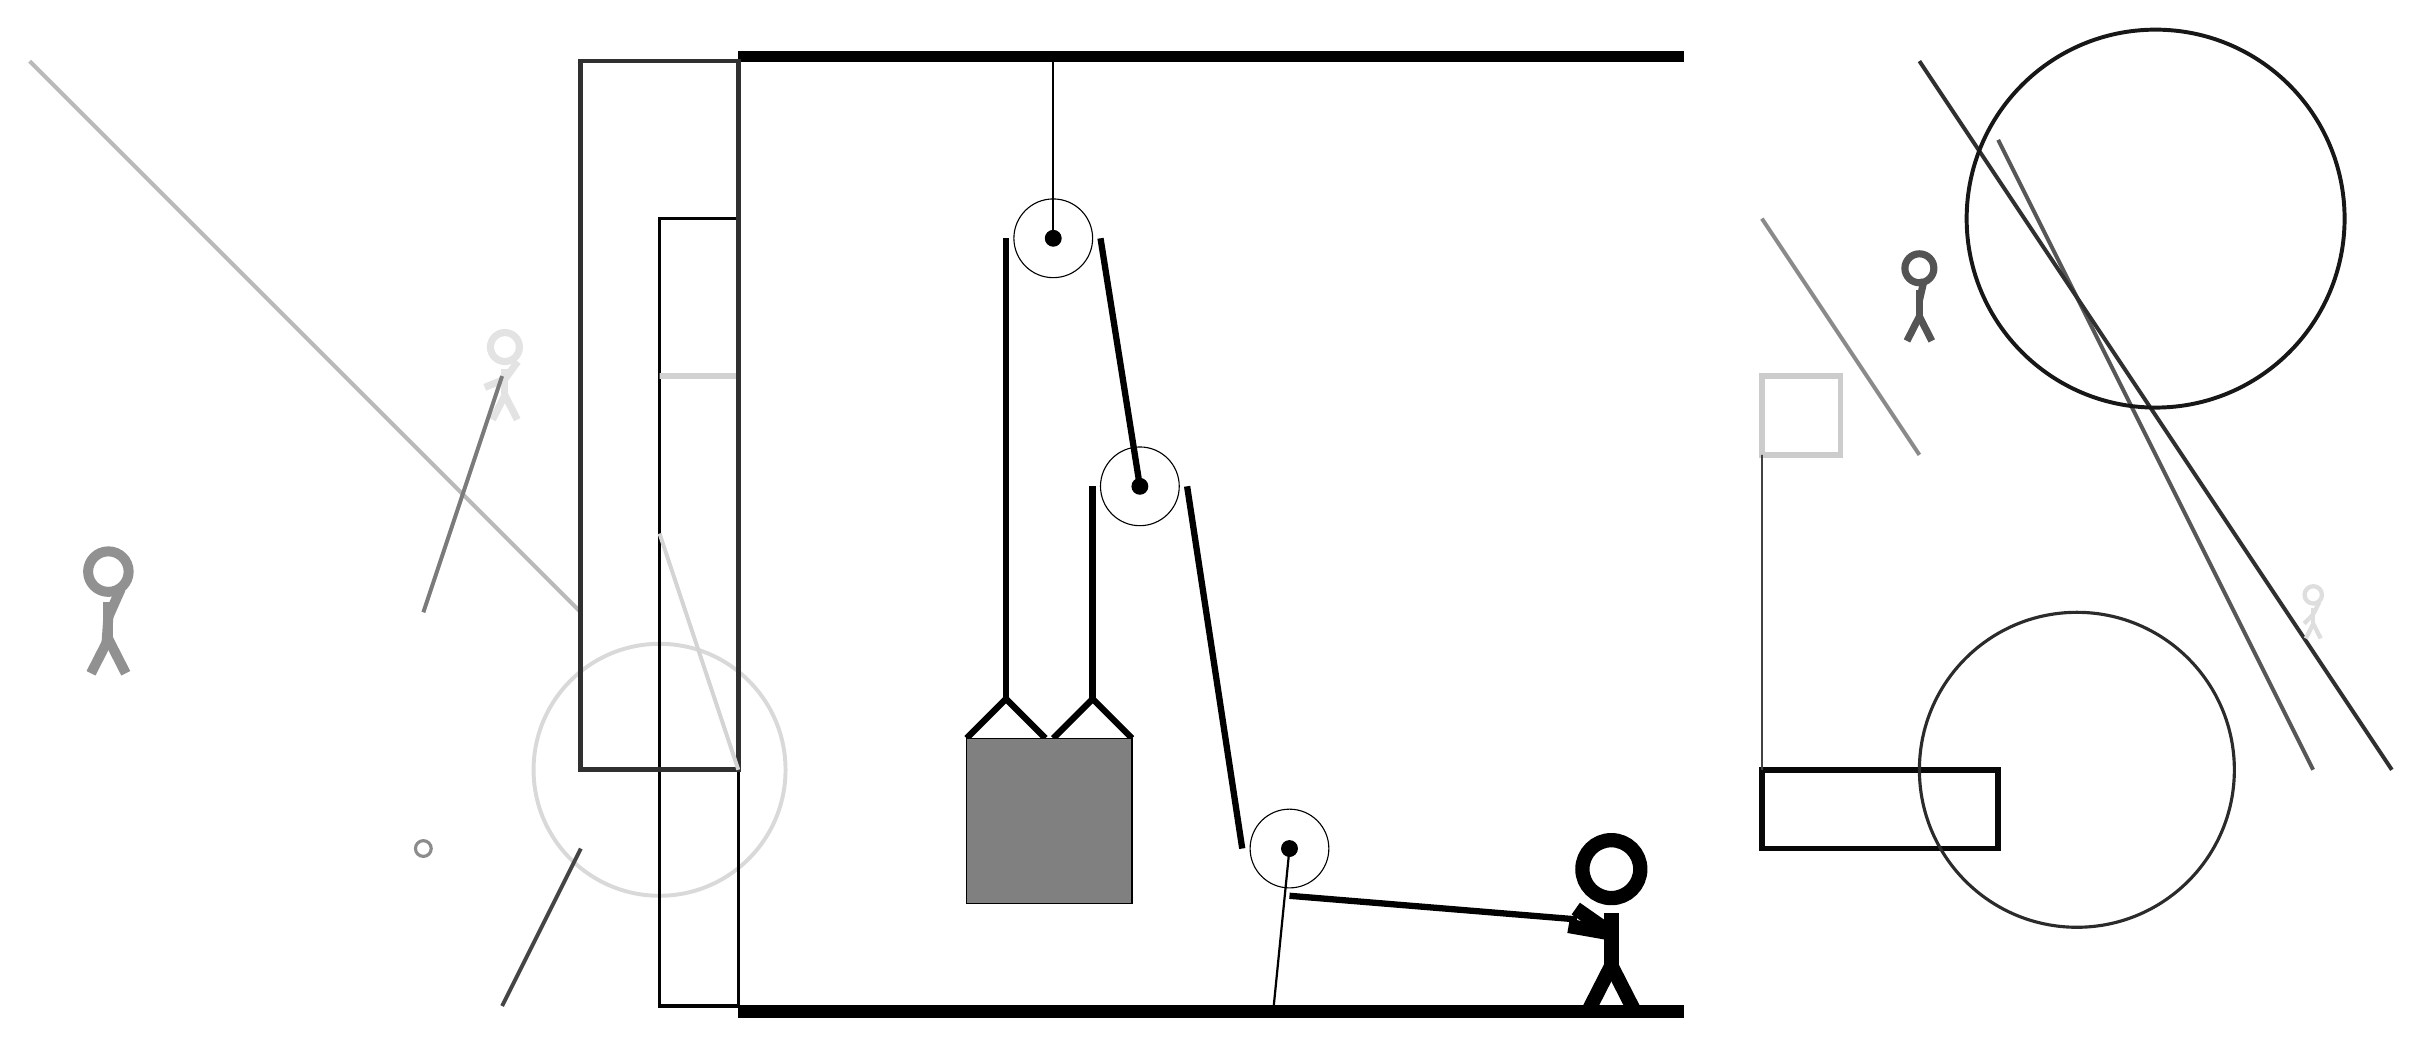
\begin{tikzpicture}
			%%%%% START %%%%%
			
			\draw[fill=black] (-2, 9) rectangle (10, 9.125);
			
			\draw[line width=0.4mm, color=black!25] (-3, 2) rectangle (-3, 4);
			
			\draw[line width=0.5mm, color=black!27](-4, 2) -- (-11, 9);
			\draw [line width=0.5mm, color=black!15](-3, 0) circle (1.6);
			\draw[line width=0.7mm, color=black!97] (11, 0) rectangle (14, -1);
			\node[line width=0.7mm, color=black!11] at (-5, 5) {\Strichmaxerl[5][22][54]};
			\draw[line width=0.5mm, color=black!66](14, 8) -- (18, 0);
			
			\node[line width=0.6mm, color=black!43] at (-10, 2) {\Strichmaxerl[7][86][66]};
			\node[line width=0.2mm, color=black!67] at (13, 6) {\Strichmaxerl[5][90][77]};
			\draw[line width=0.4mm, color=black!99] (-2, 7) rectangle (-3, -3);
			\draw[line width=0.7mm, color=black!18] (-3, 5) rectangle (-2, 5);
			\draw [line width=0.4mm, color=black!45](-6, -1) circle (0.1);
			\draw[line width=0.7mm, color=black!20] (11, 4) rectangle (12, 5);
			\draw[line width=0.5mm, color=black!81](13, 9) -- (19, 0);
			
			\draw[line width=0.6mm, color=black!81] (-2, 0) rectangle (-4, 9);
			\draw [line width=0.5mm, color=black!91](16, 7) circle (2.4);
			\draw [line width=0.4mm, color=black!83](15, 0) circle (2.0);
			
			\node[line width=0.4mm, color=black!13] at (18, 2) {\Strichmaxerl[3][46][63]};
			
			\draw[line width=0.5mm, color=black!17](-2, 0) -- (-3, 3);
			\draw[line width=0.5mm, color=black!52](-6, 2) -- (-5, 5);
			
			\draw[line width=0.3mm, color=black!74] (11, 0) rectangle (11, 4);
			\draw[line width=0.5mm, color=black!46](11, 7) -- (13, 4);
			\draw[line width=0.5mm, color=black!73](-4, -1) -- (-5, -3);
			
			\draw (2, 6.75) circle (0.5);
			\draw[fill=black] (2, 6.75) circle (0.1);
			\draw[thick] (2, 6.75) -- (2, 9);
			
			\draw (3.1, 3.6) circle (0.5);
			\draw[fill=black] (3.1, 3.6) circle (0.1);
			
			\draw (5, -1) circle (0.5);
			\draw[fill=black] (5, -1) circle (0.1);
			\draw[thick] (5, -1) -- (4.8, -3);
			
			\draw[line width = 0.8mm]  (0.9, 0.4) -- (1.4, 0.9) -- (1.9, 0.4);
			\draw[line width = 0.8mm]  (2.0, 0.4) -- (2.5, 0.9) -- (3.0, 0.4);
			\draw[fill=black!50] (0.9, 0.4) rectangle (3.0, -1.7);
			
			\draw[line width = 0.8mm] (1.4, 6.75) -- (1.4, 0.9);
			\centerarc[line width = 0.8mm](2, 6.75)(0:180:0.6);
			\draw[line width = 0.8mm] (2.6, 6.75) -- (3.1, 3.6);
			\draw[line width = 0.8mm] (2.5, 3.6) -- (2.5, 0.9);
			\centerarc[line width = 0.8mm](3.1, 3.6)(0:180:0.6);
			\draw[line width = 0.8mm] (3.7, 3.6) -- (4.4, -1);
			\centerarc[line width = 0.8mm](5, -1)(180:270:0.6);
			\draw[line width = 0.8mm] (5, -1.6) -- (8.65, -1.9);
			
			\node at (9, -2) {\Strichmaxerl[10][-35][170]};
			
			\draw[fill=black] (-2, -3) rectangle (10, -3.15);
			
			%%%%% END %%%%%
		\end{tikzpicture}
	\end{figure}	
\end{document}